\documentclass[aspectratio=169,11pt]{beamer}

% =========================================================
% PACKAGES
% =========================================================
\usepackage[T1]{fontenc}
\usepackage[utf8]{inputenc}
\usepackage{lmodern}

\usepackage{graphicx}
\usepackage{booktabs}
\usepackage{amsmath}
\usepackage{tikz}
\usepackage{ragged2e}
\usepackage{array}

\usetikzlibrary{
    arrows.meta,
    positioning,
    shapes.geometric,
    calc
}

% =========================================================
% THEME
% =========================================================
\usetheme{Boadilla}

\setbeamertemplate{navigation symbols}{}
\setbeamertemplate{headline}{}

\setbeamersize{
    text margin left=0.65cm,
    text margin right=0.65cm
}

% =========================================================
% COLORS
% =========================================================
\definecolor{mitoblue}{RGB}{31,78,121}
\definecolor{mitodark}{RGB}{36,45,55}
\definecolor{mitogray}{RGB}{105,105,105}
\definecolor{mitolight}{RGB}{245,247,249}
\definecolor{mitoline}{RGB}{215,220,225}

\setbeamercolor{normal text}{
    fg=mitodark,
    bg=white
}

\setbeamercolor{structure}{
    fg=mitoblue
}

\setbeamercolor{title}{
    fg=mitoblue
}

\setbeamercolor{subtitle}{
    fg=mitodark
}

\setbeamercolor{frametitle}{
    fg=mitoblue,
    bg=white
}

\setbeamercolor{block title}{
    bg=mitoblue,
    fg=white
}

\setbeamercolor{block body}{
    bg=mitolight,
    fg=mitodark
}

\setbeamercolor{author in head/foot}{
    bg=mitolight,
    fg=mitogray
}

\setbeamercolor{date in head/foot}{
    bg=mitolight,
    fg=mitogray
}

% =========================================================
% TYPOGRAPHY
% =========================================================
\setbeamerfont{title}{
    size=\LARGE,
    series=\bfseries
}

\setbeamerfont{subtitle}{
    size=\large
}

\setbeamerfont{author}{
    size=\normalsize
}

\setbeamerfont{institute}{
    size=\small
}

\setbeamerfont{frametitle}{
    size=\Large,
    series=\bfseries
}

\setbeamerfont{block title}{
    series=\bfseries
}

% =========================================================
% ITEMIZE
% =========================================================
\setbeamertemplate{itemize item}{
    \color{mitoblue}\small$\bullet$
}

\setbeamertemplate{itemize subitem}{
    \color{mitoblue}\scriptsize$\bullet$
}

\setlength{\leftmargini}{1.2em}
\setlength{\leftmarginii}{1.1em}

% =========================================================
% FRAME TITLE
% =========================================================
\setbeamertemplate{frametitle}{
    \vspace{0.16cm}

    \insertframetitle

    \vspace{0.06cm}

    {\color{mitoline}
    \rule{\textwidth}{0.6pt}}

    \vspace{-0.15cm}
}

% =========================================================
% FOOTER
% =========================================================
\setbeamertemplate{footline}{
    \leavevmode

    \hbox{
        \begin{beamercolorbox}[
            wd=.84\paperwidth,
            ht=2.6ex,
            dp=0.9ex,
            leftskip=1em
        ]{author in head/foot}
            MitoChime \textemdash{} NiDS2026
        \end{beamercolorbox}

        \begin{beamercolorbox}[
            wd=.16\paperwidth,
            ht=2.6ex,
            dp=0.9ex,
            center
        ]{date in head/foot}
            \insertframenumber/\inserttotalframenumber
        \end{beamercolorbox}
    }
}

% =========================================================
% DOCUMENT INFORMATION
% =========================================================
\title{MitoChime}

\subtitle{
    A Machine Learning Pipeline for Detecting PCR-Induced Chimeras\\
    in Mitochondrial Illumina Reads
}

\author{
    Yvonne Lin \quad
    Duranne Duran \quad
    Daniella Pailden \quad
    Francis Dimzon
}

\institute{
    University of the Philippines Visayas
}

\date{NiDS2026}

% =========================================================
% DOCUMENT
% =========================================================
\begin{document}

% =========================================================
% SLIDE 1 — TITLE
% =========================================================
\begin{frame}[plain]

    \vfill

    \begin{center}

        {\usebeamerfont{title}
        \color{mitoblue}
        \inserttitle
        \par}

        \vspace{0.35cm}

        {\usebeamerfont{subtitle}
        \color{mitodark}
        \insertsubtitle
        \par}

        \vspace{0.8cm}

        {\usebeamerfont{author}
        Yvonne Lin \quad
        Duranne Duran \quad
        Daniella Pailden \quad
        Francis Dimzon
        \par}

        \vspace{0.35cm}

        {\usebeamerfont{institute}
        University of the Philippines Visayas
        \par}

        \vspace{0.45cm}

        {\small
        \color{mitogray}
        NiDS2026
        }

    \end{center}

    \vfill

\end{frame}


% =========================================================
% PRESENTER 1 — INTRODUCTION
% =========================================================

% ---------------------------------------------------------
% SLIDE 2 — PCR-INDUCED CHIMERAS
% ---------------------------------------------------------

% To be added.


% ---------------------------------------------------------
% SLIDE 3 — RESEARCH GAP AND OBJECTIVE
% ---------------------------------------------------------

% To be added.



% =========================================================
% PRESENTER 2 — METHODOLOGY
% =========================================================

% ---------------------------------------------------------
% SLIDE 4 — EXPERIMENTAL SETUP
% ---------------------------------------------------------
\begin{frame}{Experimental Setup}

\vspace{0.02cm}

\begin{center}

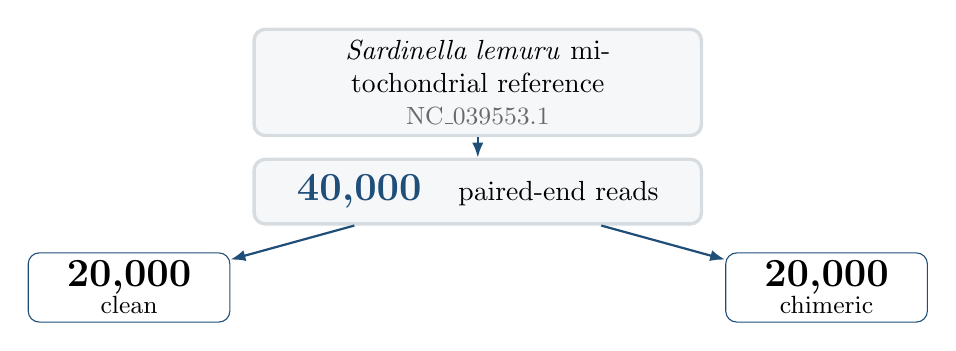
\begin{tikzpicture}[
    mainbox/.style={
        draw=mitoline,
        very thick,
        rounded corners=4pt,
        fill=mitolight,
        align=center,
        minimum height=0.82cm,
        text width=5.4cm,
        inner sep=4pt
    },
    splitbox/.style={
        draw=mitoblue,
        rounded corners=4pt,
        fill=white,
        align=center,
        minimum height=0.82cm,
        text width=2.35cm,
        inner sep=3pt
    },
    flowarrow/.style={
        -{Latex[length=1.9mm]},
        thick,
        draw=mitoblue
    }
]

\node[mainbox] (reference) {
    \textit{Sardinella lemuru} mitochondrial reference\\[-0.02cm]
    {\small\color{mitogray}NC\_039553.1}
};

\node[
    mainbox,
    below=0.26cm of reference
] (dataset) {
    {\Large\color{mitoblue}\textbf{40,000}}
    \quad paired-end reads
};

\node[
    splitbox,
    below left=0.34cm and 0.28cm of dataset
] (clean) {
    {\Large\textbf{20,000}}\\[-0.08cm]
    {\small clean}
};

\node[
    splitbox,
    below right=0.34cm and 0.28cm of dataset
] (chimera) {
    {\Large\textbf{20,000}}\\[-0.08cm]
    {\small chimeric}
};

\draw[flowarrow] (reference) -- (dataset);
\draw[flowarrow] (dataset) -- (clean);
\draw[flowarrow] (dataset) -- (chimera);

\end{tikzpicture}

\end{center}

\vspace{0.30cm}

\begin{columns}[T,onlytextwidth]

    \begin{column}{0.31\textwidth}
        \centering

        {\Large\color{mitoblue}\textbf{150 bp}}\\[0.04cm]
        {\small Read length}
    \end{column}

    \begin{column}{0.31\textwidth}
        \centering

        {\Large\color{mitoblue}\textbf{80 / 20}}\\[0.04cm]
        {\small Train / held-out test}
    \end{column}

    \begin{column}{0.31\textwidth}
        \centering

        {\Large\color{mitoblue}\textbf{5-fold}}\\[0.04cm]
        {\small
        Stratified cross-validation\\[-0.02cm]
        on the training split
        }
    \end{column}

\end{columns}

\end{frame}


% ---------------------------------------------------------
% SLIDE 5 — MITOCHIME WORKFLOW
% ---------------------------------------------------------
\begin{frame}{MitoChime Workflow}

\vspace{0.55cm}

\begin{center}

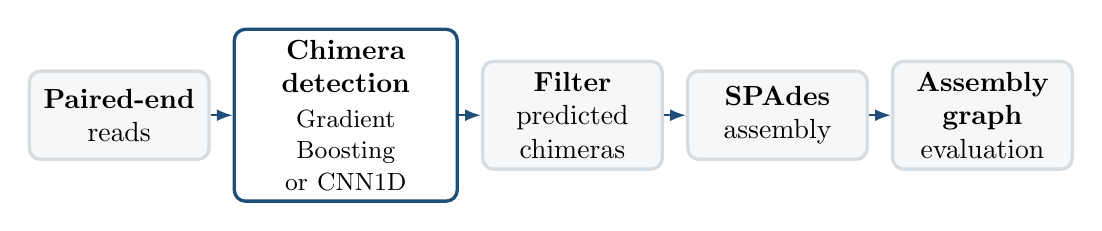
\begin{tikzpicture}[
    node distance=0.28cm,
    workflow/.style={
        draw=mitoline,
        very thick,
        rounded corners=4pt,
        fill=mitolight,
        align=center,
        minimum height=1.12cm,
        text width=2.0cm,
        inner sep=4pt
    },
    detection/.style={
        workflow,
        draw=mitoblue,
        fill=white,
        text width=2.55cm
    },
    flowarrow/.style={
        -{Latex[length=2mm]},
        thick,
        draw=mitoblue
    }
]

\node[workflow] (reads) {
    \textbf{Paired-end}\\
    reads
};

\node[
    detection,
    right=of reads
] (detect) {
    \textbf{Chimera detection}\\[0.06cm]
    {\small
    Gradient Boosting\\[-0.02cm]
    or CNN1D
    }
};

\node[
    workflow,
    right=of detect
] (filter) {
    \textbf{Filter}\\
    predicted chimeras
};

\node[
    workflow,
    right=of filter
] (assembly) {
    \textbf{SPAdes}\\
    assembly
};

\node[
    workflow,
    right=of assembly
] (evaluate) {
    \textbf{Assembly graph}\\
    evaluation
};

\draw[flowarrow] (reads) -- (detect);
\draw[flowarrow] (detect) -- (filter);
\draw[flowarrow] (filter) -- (assembly);
\draw[flowarrow] (assembly) -- (evaluate);

\end{tikzpicture}

\end{center}

\vspace{0.70cm}

\begin{center}
    \large
    Predicted chimeric reads are removed
    \textbf{before assembly}.
\end{center}

\vspace{0.18cm}

\begin{center}
    \small
    \color{mitogray}
    Downstream impact is evaluated through the resulting
    assembly graph structure.
\end{center}

\end{frame}


% ---------------------------------------------------------
% SLIDE 6 — TWO DETECTION APPROACHES
% ---------------------------------------------------------
\begin{frame}{Two Approaches to Chimera Detection}

\vspace{0.15cm}

\begin{columns}[T,onlytextwidth]

% =========================================================
% LEFT — GRADIENT BOOSTING
% =========================================================
\begin{column}{0.48\textwidth}

    \begin{center}
        {\large\color{mitoblue}\textbf{Gradient Boosting}}\\[0.02cm]
        {\small\color{mitogray}Feature-based}
    \end{center}

    \vspace{0.18cm}

    \begin{center}

    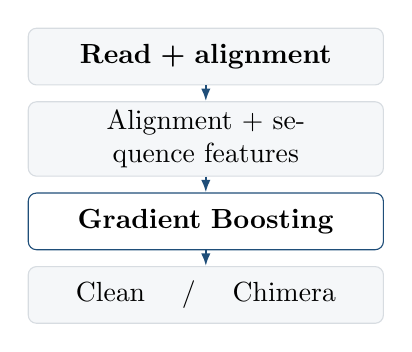
\begin{tikzpicture}[
        node distance=0.20cm,
        box/.style={
            draw=mitoline,
            rounded corners=3pt,
            fill=mitolight,
            align=center,
            minimum height=0.72cm,
            text width=4.3cm,
            inner sep=3pt
        },
        model/.style={
            box,
            draw=mitoblue,
            fill=white
        },
        arrow/.style={
            -{Latex[length=1.6mm]},
            thick,
            draw=mitoblue
        }
    ]

    \node[box] (input) {
        \textbf{Read + alignment}
    };

    \node[box, below=of input] (features) {
        Alignment + sequence features
    };

    \node[model, below=of features] (gb) {
        \textbf{Gradient Boosting}
    };

    \node[box, below=of gb] (output) {
        Clean \quad / \quad Chimera
    };

    \draw[arrow] (input) -- (features);
    \draw[arrow] (features) -- (gb);
    \draw[arrow] (gb) -- (output);

    \end{tikzpicture}

    \end{center}

    \vspace{0.22cm}

    \begin{center}
        {\small\color{mitogray}
        Examples of extracted signals
        }

        \vspace{0.10cm}

        {\small
        \textbf{Alignment structure}
        \quad $\bullet$ \quad
        \textbf{Clipping}
        }

        \vspace{0.07cm}

        {\small
        \textbf{6-mer discontinuity}
        \quad $\bullet$ \quad
        \textbf{Microhomology}
        }
    \end{center}

\end{column}


% =========================================================
% RIGHT — CNN1D
% =========================================================
\begin{column}{0.48\textwidth}

    \begin{center}
        {\large\color{mitoblue}\textbf{CNN1D}}\\[0.02cm]
        {\small\color{mitogray}Sequence-based}
    \end{center}

    \vspace{0.18cm}

    \begin{center}

    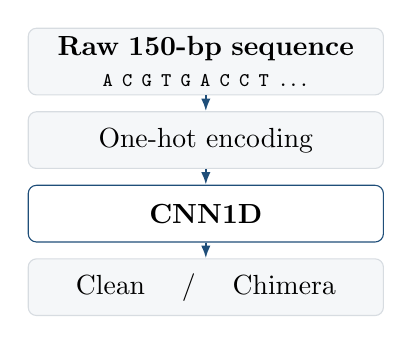
\begin{tikzpicture}[
        node distance=0.20cm,
        box/.style={
            draw=mitoline,
            rounded corners=3pt,
            fill=mitolight,
            align=center,
            minimum height=0.72cm,
            text width=4.3cm,
            inner sep=3pt
        },
        model/.style={
            box,
            draw=mitoblue,
            fill=white
        },
        arrow/.style={
            -{Latex[length=1.6mm]},
            thick,
            draw=mitoblue
        }
    ]

    \node[box] (input) {
        \textbf{Raw 150-bp sequence}\\[-0.03cm]
        {\scriptsize\texttt{A C G T G A C C T \ldots}}
    };

    \node[box, below=of input] (encoding) {
        One-hot encoding
    };

    \node[model, below=of encoding] (cnn) {
        \textbf{CNN1D}
    };

    \node[box, below=of cnn] (output) {
        Clean \quad / \quad Chimera
    };

    \draw[arrow] (input) -- (encoding);
    \draw[arrow] (encoding) -- (cnn);
    \draw[arrow] (cnn) -- (output);

    \end{tikzpicture}

    \end{center}

    \vspace{0.22cm}

    \begin{center}
        {\small\color{mitogray}
        Learns sequence patterns directly
        }

        \vspace{0.10cm}

        {\small
        \textbf{3 convolutional blocks}
        }

        \vspace{0.07cm}

        {\small
        64 $\rightarrow$ 128 $\rightarrow$ 256 filters
        }
    \end{center}

\end{column}

\end{columns}

\end{frame}



% =========================================================
% PRESENTER 3 — RESULTS AND CONCLUSION
% =========================================================

% ---------------------------------------------------------
% SLIDE 7 — CLASSIFICATION PERFORMANCE
% ---------------------------------------------------------

% To be added.


% ---------------------------------------------------------
% SLIDE 8 — ASSEMBLY RESULTS
% ---------------------------------------------------------

% To be added.


% ---------------------------------------------------------
% SLIDE 9 — CONCLUSION
% ---------------------------------------------------------

% To be added.


\end{document}